%!TEX root = ../presentation.tex

\begin{frame}{Examples}
    \textbf{Example: Triaxial compression test}
\begin{minipage}{1.0\textwidth}
\begin{minipage}{0.55\textwidth}
    \begin{itemize}
        \item Cylindrical specimen
        \item Subjected to axial displacement controlled compression
        \item Different confining pressures (0, 2.5 and 5.0 MPa)
        \item Evolving shear band in the center of the specimen
        \item Gradient-Enhanced Drucker-Prager model
    \end{itemize}
\end{minipage}\hfill{}%
\begin{minipage}{0.4\textwidth}
    \centering
    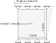
\includegraphics[width=1.0\linewidth]{\slidedir/setup.pdf}
\end{minipage}
\end{minipage}
% \vspace{2em}
\vfill

\begin{minipage}{1.0\textwidth}
    \begin{figure}[htpb]
        \centering
    \includegraphics[height=3cm]{\slidedir/p0_warp15_nonlocaldmg_cropped.png}%
    \hspace{1cm}%
    \includegraphics[height=3cm]{\slidedir/p2,5_warp5_nonlocaldmg_cropped.png}%
    \hspace{1cm}%
    \includegraphics[height=3cm]{\slidedir/p5,0_warp5_nonlocaldmg_cropped.png}%
    \caption{Predicted damage: Uniaxial compression (left), 2.5 MPa confing pressure (center), 5.0 MPa confining pressure (right).} 
        \label{fig:name}
    \end{figure}
\end{minipage}
\end{frame}
